\documentclass[12pt]{article}

\usepackage[utf8]{inputenc}
\usepackage[margin=0.6in]{geometry}

\usepackage{amsmath}
\usepackage{graphicx}
\usepackage{booktabs}

\newcommand{\D}[2]{\frac{\mathrm{d}#1}{\mathrm{d}#2}}
\newcommand{\pfrac}[2]{\left(\frac{#1}{#2} \right)}
\newcommand{\ex}[1]{\left\langle#1\right\rangle}

\begin{document}

\section{Lane-Emden Equation and Polytropes}

\subsection*{a}

First distribute the outer derivative in the Lane-Emden equation and then multiply through by \(\xi^2\):

\[ 2\theta'+\xi\theta'' + \xi\theta_n^n = 0
\]

Substitute the Taylor series \( \theta_n= \sum\limits_{k=0}^\infty a_k \xi^k \) and \( \theta_n^n= \sum\limits_{k=0}^\infty c_k \xi^k \) (written this way to avoid typing a lot of derivatives evaluated at \(\xi=0\)) to find\\

\[\sum\limits_{k=1}^\infty 2a_k k \xi^{k-1}  + \sum\limits_{k=2}^\infty k(k-1)a_k \xi^{k-1} +  \sum\limits_{k=0}^\infty c_k \xi^{k+1} = 0
\]\\

We have \(\theta'(0) = 0\) as a boundary condition, so we know \(a_1 = 0\), and the first sum can start from \(k=2\). Shifting the index on the last sum,

\[ \sum\limits_{k=2}^\infty \left(2a_{k}k +a_k k(k-1) + c_{k-2}\right)\xi^{k-1} = 0
\]

The \(c_k\)'s are pretty tedious to compute in terms of the \(a_k\)'s, but the first few are easy. Recalling \(a_0 = 1\) is a boundary condition, it's obvious that \(  \left(a_0+a_1\xi+ a_2\xi^2\right)^n = \left( 1+a_2\xi^2 \right)^n = 1 + a_2 n \xi^2 + O(\xi^4)\), which yields \(c_0 = 1\), \(c_1 = 0\), and \(c_2 = na_2\). Substituting into the above up to \(k=4\), we end up with the system

\begin{align*}
6a_2 + 1 &= 0\\
12a_3 &= 0\\
20a_4 + na_2 &= 0
\end{align*}

This gives \(a_2 = -\frac{1}{6}\), \(a_3 = 0\), and \(a_4 = \frac{n}{120}\), whence we can claim near \(\xi=0\) that

\[ \theta \approx 1 - \frac{1}{6}\xi^2 + \frac{n}{120}\xi^4
\]

I remember somewhere that there should be a recurrence relation for \(c_k\). In principle we could substitute that instead into the above and probably get a recurrence relation for \(a_k\). I'm willing to guess though that the recurrence for \(c_k\) is complicated, or else everyone would have memorized it, since having the coefficients of a power of a power series is a really generally useful thing.

\subsection*{b}

Let's just write the obvious formula for enclosed mass and start changing variables until we get what we're looking for.

\begin{align*}
m = \int_0^r 4\pi r^3\rho\mathrm{dr} = \int_0^{r}4\pi r_n^3 \xi^3 \rho_c \theta^n_n \mathrm{dr} = 4\pi r_n^3 \rho_c\int_0^{\xi}\xi'^2\theta_n^n\mathrm{d\xi'}
\end{align*}

Integrating over \(\theta^n\) looks like a bad idea, but we can substitute for it from the Lane-Emden equation:

\[ m = -4\pi \rho_c r_n^3 \int_0^{\xi} \frac{\mathrm{d}}{\mathrm{d\xi'}}\left(\xi'^2\frac{\mathrm{d\theta_n}}{\mathrm{d\xi'}} \right)\mathrm{d\xi'} = -4\pi\rho_c r_n^3 \xi^2 \frac{\mathrm{d\theta_n}}{\mathrm{d\xi}}
\]

\subsection*{c}

Expand out the \(r_n\) in our expression for \(m\):

\[ M = -4\pi\rho_c^{1+\frac{3(1-n)}{2n}}\xi_1^2 \frac{\mathrm{d}\theta_n(\xi_1)}{\mathrm{d}\xi} \left( \frac{(n+1)K}{4\pi G} \right)^{3/2} = -4\pi\rho_c^{\frac{3-n}{2n}} \left( \frac{(n+1)K}{4\pi G} \right)^{3/2}\xi_1^2\frac{\mathrm{d}\theta_n(\xi_1)}{\mathrm{d}\xi}
\]

So we can substitute an expression for \(\rho_c\) into \(r=r_n \xi\):

\begin{align*}
\rho_c &= \left(-\frac{M}{4\pi}\left(\frac{(n+1)K}{4\pi G}\right)^{-3/2}\left(\xi_1^2\frac{\mathrm{d}\theta_n(\xi_1)}{\mathrm{d}\xi}\right)^{-1}\right)^{\frac{2n}{3-n}}\\
R &= \left(-\frac{M}{4\pi}\left(\frac{(n+1)K}{4\pi G}\right)^{-3/2}\left(\xi_1^2\frac{\mathrm{d}\theta_n(\xi_1)}{\mathrm{d}\xi}\right)^{-1}\right)^{\frac{1-n}{3-n}} \pfrac{(n+1)K}{4\pi G}^{1/2} \xi_1
%R &= r_n \xi_1 = \left( \frac{-(n+1)K}{4\pi G} \right)^\frac{n}{3-n} \left(\xi_1^2\frac{\mathrm{d}\theta_n(\xi_1)}{\mathrm{d}\xi}\right)^{\frac{n-1}{3-n}}M^{\frac{1-n}{3-n}}
\end{align*}

So \(RM^{\frac{n-1}{3-n}}\) is a constant. For \(n=3/2\), this is \(RM^{1/3}\). Equivalently, \(MR^3\) is constant.

\subsection*{d}

From the first line in (c), \(M\propto \rho_c^{\frac{3-n}{2n}}\), so for \(n=3\) we have \(M\propto \rho_c^0\).

\subsection*{e}

See the attached notebook for implementation. There are two numerical integrators. One is a very self explanatory Euler integrator, and the other is the RK4 recipe from HWT chapter 7 which determines initial conditions from the taylor expansion of the Lane-Emden equation about the origin. Their results differ negligibly for our purposes here (not shown, but quick to see with the notebook open). All results quoted are from the RK4 integrator.

\begin{center}
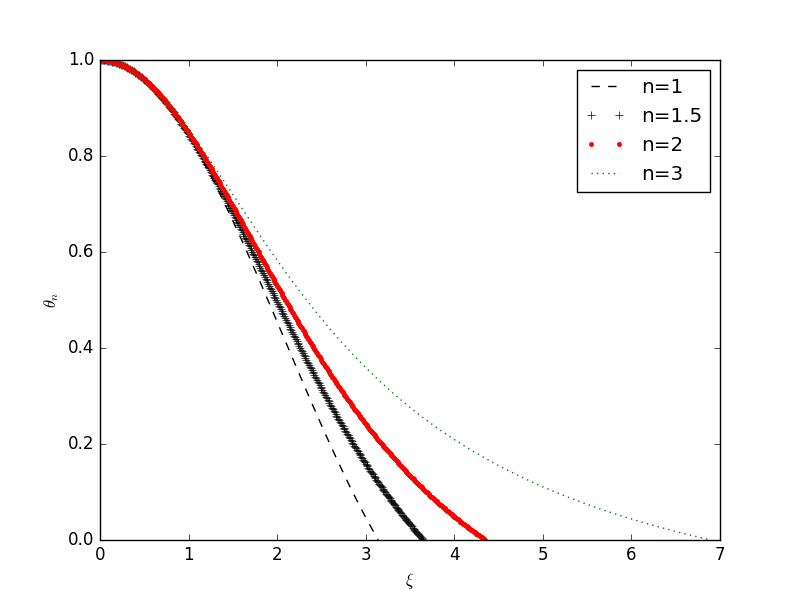
\includegraphics[scale=.5]{theta_xi.png}
\end{center}


\begin{center}

\begin{tabular}{ccc}
\toprule
   n &   \( \xi_1 \) &  \( \frac{d\theta_n (\xi_1)}{d\xi} \) \\
\midrule
 1.0 &      3.141501 &                             -0.318306 \\
 1.5 &      3.653601 &                             -0.203305 \\
 2.0 &      4.352801 &                             -0.127246 \\
 3.0 &      6.896901 &                             -0.042428 \\
\bottomrule
\end{tabular}

\end{center}

\subsection*{f}

Right away we can write

\begin{align*}
&P_{\mathrm{gas}} = \beta P = \frac{kT}{\mu m_H}\rho\\
&P_{\mathrm{rad}} = (1-\beta)P = \frac{1}{3}aT^4
\end{align*}

This yields for temperature

\[ T = (3(1-\beta)P/a)^{1/4} = \mu\beta m_H P / \rho k
\]

which yields for P,

\[ P^{-3} = \frac{a}{3(1-\beta)}\left(\frac{\mu m_H \beta}{\rho k}  \right)^4
\]

or

\[ P =  \pfrac{3}{a}^{1/3}  \pfrac{k}{\mu m_H}^{4/3} \pfrac{1-\beta}{\beta^4}^{1/3}  \rho^{4/3}
\]

\subsection*{g}

It fortunately happens that for \(n=3\), our expression for \(M\) in (c) becomes independent of \(\rho_c\):

\[ M = 4\pi \pfrac{K}{\pi G}^{3/2} D_3
\]

where \(D_3 = -\xi_1^2\frac{\mathrm{d}\theta_3(\xi_1)}{\mathrm{d}\xi}\). We also have from (f),

\[ K =  \pfrac{3}{a}^{1/3}  \pfrac{k}{\mu m_H}^{4/3} \pfrac{1-\beta}{\beta^4}^{1/3}
\]\\

Eliminating \(K\) from the latter and solving for \( (1-\beta)/\mu^4\beta^4\),

\[ \frac{1-\beta}{\mu^4\beta^4} = \pfrac{M}{\sqrt{48k^4D_3^2/m_H^4 G^3\pi a} }^2
\]\\

Hopefully the denominator is \(M_{\mathrm{edd}}\). Anyway, we can evaluate it:

\[ M_{\mathrm{edd}} = 1.77 \times 10^{31} D_3 \, \mathrm{kg}
\]

\(D_3\) we find from numerical integration to be 2.018, so \(M_{\mathrm{edd}}\) comes out to about eighteen solar masses.

\subsection*{h}

Suppose we're dealing with a fully ionized material. We expect that the number density of particles due to hydrogen will be approximately \(n_X = 2X\rho/m_H\), because we get about two particles per hydrogen mass since \(m_H \approx m_p\). Helium has an atomic mass number close to four, so ionizing \(4m_H\) of helium yields three particles (two electrons and a helium nucleus), and we expect \(n_Y = 3Y\rho/4m_H\). Heavier elements tend to have half as many electrons as nucleons, and should roughly tend toward \(n_Z = Z\rho/2m_H\).

Then \(\rho = \mu n m_H  = \mu m_H (8X +3Y + 2Z)\rho/4m_H\) so that \(\mu = 4/(8X+3Y+2Z)\). Since \(Z=1-X-Y\), this simplifies to \(\mu=4/(6X+Y+2)\). For the values given, this yields

\[\mu = .603\]

Then using a numerical solver,

\[ \frac{1-\beta}{(.603)^4 \beta^4} \approx 1/18^2 \implies \beta \approx 1 - (4 \times 10^{-4})
\]


We're given the stellar radius, so we can get the central density from \(R = r_n \xi_1\):

\[ \rho_c = \left( \pfrac{\pi G}{K}^{1/2} \frac{R}{\xi_1}  \right) ^ {\frac{2n}{1-n}}
\]



We can get the core temperature by looking back at (f):

\[ T_c = \frac{\mu \beta m_H P_c}{k\rho_c}
\]

The central pressure is just \(P_c = K \rho_c^{4/3}\). Since \(\beta\approx 1\), almost all of this is in gas pressure.

Finally, all we need to evaluate it is to evaluate K:

\begin{align*}
K &= \pfrac{3}{a}^{1/3} \pfrac{k}{m_H}^{4/3} \pfrac{1-\beta}{\mu^4 \beta^4}^{1/3} \\[7pt]
&= \pfrac{3}{a}^{1/3} \pfrac{k}{m_H}^{4/3} \pfrac{1}{18^2}^{1/3} \\[7pt]
&= 3.84 \times 10^{14} \, \mathrm{dyne} \, \mathrm{g}^{-3/4} \,\mathrm{cm}^{-1/4}
\end{align*}

Consolidating results into one place,

\begin{align*}
T_c &= 1.19 \times 10^{7} \, \mathrm{K} \\
\rho_c &= 76.35 \, \mathrm{g}\,\mathrm{cm}^{-3} \\
P_c &= 1.2437 \times 10^{17} \, \mathrm{dyne} \, \mathrm{cm}^{-2}
\end{align*}

So we're low on all of these by a factor of order unity. \(\mu\) is probably higher than the average of .6 as we approach the core as we become more hydrogen depleted, so this is probably expected.

\subsection*{i}

This is an index 3 polytrope with mass

\[ 4\pi \pfrac{K}{\pi G}^{3/2} D_3
\]

and

\[ K = \frac{2\pi hc}{3} \pfrac{3Z}{8\pi A m_p}^{4/3}
\]

Using \(D_3 = 2.018\) and \(Z/A=.5\), the mass evaluates to \(M_{ch} = 7.48 M_{\odot}\). This is just not my day for getting the numerics to come out right.

\section{Degenerate Matter}

\subsection*{a}

We can do this integral in phase space directly. Let \(f_F = f(p)\) on \([0,p_F]\), where \(p_f = \sqrt{2m\varepsilon_F}\). We have

\begin{align*}
n = \int_0^{p_F} f(p) g_d \mathrm{d^3 p} &= f_p g_d \frac{4}{3}\pi p_F^3\\
&= \frac{8\pi}{3}(2m\varepsilon_F)^{3/2}f_p\\
&\implies f_p = \frac{3n}{8\pi}(2m\varepsilon_F)^{-3/2}
\end{align*}

\subsection*{b}

\begin{align*}
\ex{E} &= \int_0^{\varepsilon_F} \frac{3}{8\pi}(2m\varepsilon_F)^{-3/2} E \mathrm{dE} = \frac{3}{16\pi}(2m\varepsilon_F)^{-3/2}\varepsilon_F^2\\[10pt]
\ex{v} &= \int_0^{\varepsilon_F} \frac{3}{8\pi}(2m\varepsilon_F)^{-3/2}\sqrt{\frac{2E}{m}} \mathrm{dE} = \frac{1}{4\pi}\sqrt{\frac{2}{m}}(2m\varepsilon_F)^{-3/2} \varepsilon_F^{3/2} = \frac{1}{8\pi m^2}\\[10pt]
\ex{P} &= \int_0^{\varepsilon_F} \frac{3}{8\pi}(2m\varepsilon_F)^{-3/2} \frac{2nE}{3} \mathrm{dE} = \frac{n}{8\pi}(2m\varepsilon_F)^{-3/2}\varepsilon_F^2
\end{align*}

\subsection*{c}

Let's just substitute \(\varepsilon_F\) into our expression for \(\ex{P}\):

\begin{align*}
\ex{P} &= \frac{n}{8\pi}(2m)^{-3/2}\varepsilon_F^{1/2} = \frac{n}{8\pi}(2m)^{-3/2}\frac{\hbar}{\sqrt{2m}}(3\pi^2n)^{1/3} = \frac{\hbar\sqrt[3]{3\pi^2}}{32\pi m^2}n^{4/3} \\
&= \frac{\hbar\sqrt[3]{3\pi^2}}{32\pi m^{10/3}}\rho^{4/3}
\end{align*}

I'm not sure where to find the missing factor of \(n^{1/3}\).

\subsection*{d}

Recall from the last equation of (1c) that for n=1.5 \( R \propto KM^{-1/3}\). For a nonrelativistic degenerate fermi gas, K goes with \(\mu^{-5/3}\), and we have \(R \propto \mu^{-5/3}M^{-1/3}\) and it follows immediately that for two nonrelativistic degenerate fermi gases a and b,

\[ \frac{R_a}{R_b} = \pfrac{\mu_b}{\mu_a}^{5/3}\pfrac{M_b}{M_a}^{1/3}
\]\\

Using (1h), we can take the white dwarf to have \(Z\approx 1\) to find \(\mu_{\mathrm{WD}} = 2\). Previously we found \(\mu_{\mathrm{sun}} \approx .6\). We get 

\[ \frac{R_{\mathrm{WD}}}{R_{\mathrm{BD}}} = \pfrac{.6}{2}^{5/3} \pfrac{.1}{1}^{1/3} \approx .06
\]


\section{Minimum mass for hydrogen fusion}

\subsection*{a}

%\(R = \frac{(5/2)K D_{3/2}}{4\pi G}\xi_1M^{-1/3}\)

\(n=3/2\) again and \(R=\frac{5K}{8\pi G}\pfrac{M}{4\pi D_{3/2}}^{-1/3}\xi_1\). We're given \(K \approx 10^{13}\left( 1 + \eta + \frac{\eta^2}{1+\eta}\right)\). Using \(D_{3/2} = 2.714\) and \(\xi_1 = 3.6536\) from our numerical integrator,

\[ R = (3.53 \times 10^{20})\left( 1 + \eta + \frac{\eta^2}{1+\eta}\right) \pfrac{1}{M}^{1/3}
\]

Pulling out a factor of \((2\times 10^{33})^{-1/3}\) gives

\[ R_0 = 2.807 \times 10^ {9} \pfrac{M_{\odot}}{M}^{1/3} \, \mathrm{cm}
\] 


\subsection*{b}


Evaluating using \(R_0 = 2.8 \times 10^9\) cm gives \(\eta \approx .143\).


\subsection*{c}

Insert the expression for \(\eta\) into the expression for \(R\):

\[ R = \left( 1 + \alpha T_c R^2 + \frac{\alpha^2 T_c^2 R^4}{1+\alpha T_c R^2}\right)R_0
\]

where \(\alpha = 10^{-9}\pfrac{M_{\odot}}{M}^{4/3}R_0^{-2}\). This gives \(T_c\) as an implicit function of \(R\):



\subsection*{d}

\[ M = \pfrac{T_c}{2\times 10^{8}}^{3/4}M_{\odot}
\]

For \(T_c = 3 \times 10^6\) K, this is \(.043\,M_{\odot}\), which is an impressively small mass for hydrogen burning.


\end{document}